
\documentclass{beamer} 
\usetheme{Singapore}

\usepackage[utf8]{inputenc}
\usepackage[portuguese]{babel}
\usepackage{underscore}
\usepackage{lmodern}
\usepackage[absolute,overlay]{textpos} 
\newenvironment{reference}[2]{% 
  \begin{textblock*}{\textwidth}(#1,#2) 
      \footnotesize\it\bgroup\color{red!50!black}}{\egroup\end{textblock*}} 
\title{Funtoo/Gentoo o mundo da flexibilidade e alto despenho no Linux}
\author[Lopez. V.L.O]{Víctor Orozco @tuxtor}
\date{\today}

\begin{document}
\begin{frame}[Plain]
\titlepage
\end{frame}

\begin{frame}{Roteiro}
\frametitle{Roteiro}
\tableofcontents
\end{frame} 

\section{Distros GNU/Linux}
\begin{frame}{Distribuiçoes GNU/Linux}
\begin{center}
Quantas distribuições existem na actualidade?
\end{center}
\begin{figure}[tbph]
\centering

\includegraphics[width=0.3\linewidth]{./question}
\label{fig:question}
\end{figure}
\end{frame}

\begin{frame}{Distribuiçoes GNU/Linux}
\begin{figure}[tbph]
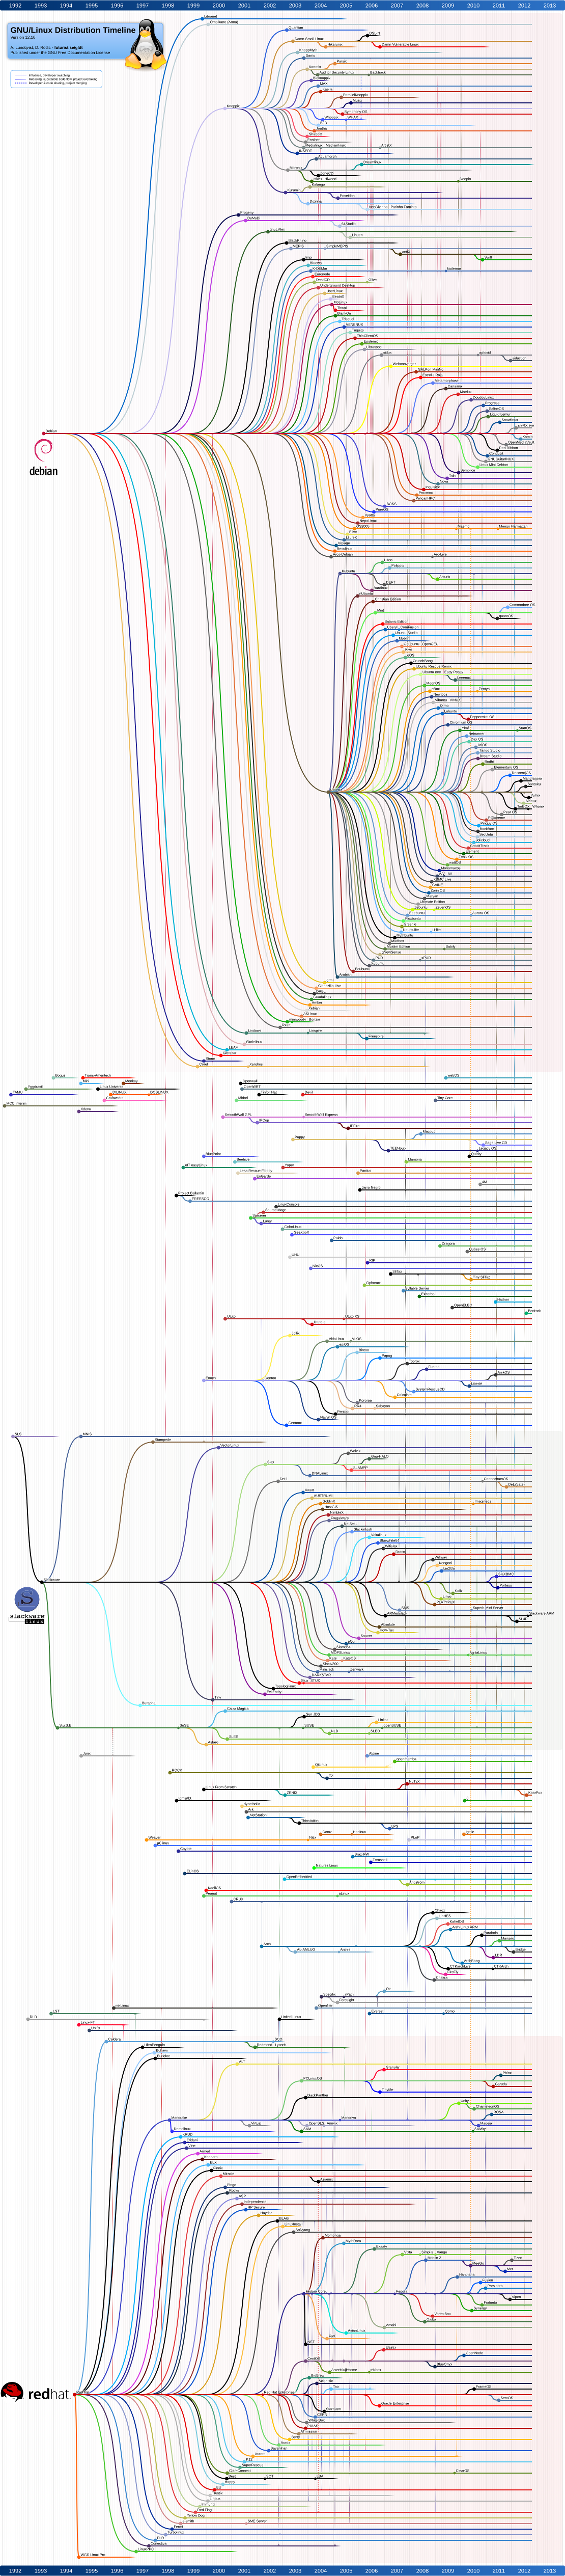
\includegraphics[height=0.95\textheight]{./gldt1210}
\end{figure}
\end{frame}

\begin{frame}{Distribuiçoes GNU/Linux}
\begin{itemize}
\item De acordo com o timeline de distribuições GNU/Linux \cite{GDT2012} aprox. 450 . . . sim 450 e contando!
\item Podem ser identificadas distribuições raiz, algumas das mais famosas \cite{YoLinux012}
\begin{itemize}
\item Red Hat
\item Debian
\item Suse
\item Gentoo
\item Slackware
\item Arch
\end{itemize}
\end{itemize}
\end{frame}

\begin{frame}{Distribuiçoes Linux}
\begin{center}
Qual e a diferença entre elas?
\end{center}
\begin{figure}[tbph]
\centering

\includegraphics[width=0.3\linewidth]{./question}
\label{fig:question2}
\end{figure}
\end{frame}

\begin{frame}{Distribuiçoes GNU/Linux}
\begin{enumerate}
\item Cores e papel de parede
\item Conjunto de pacotes incluídos na distribuição
\item Software original da distribuição
\item Estrutura interna da distribuição (pastas, arquivos de configuração)
\item Gestores de pacotes (gestor de dependências e instalador)
\end{enumerate}
\end{frame}

\section{Pacotes}
\begin{frame}{Formatos de pacotes}
\begin{itemize}
\item Baseados em binários
\begin{itemize}
\item .deb (Ubuntu,Debian,MacOS(Fink))
\item .rpm (Red Hat, Mandriva)
\item .tgz (Arch, Slackware)
\end{itemize}
\item Baseados em código fonte
\begin{itemize}
\item spells (Sorcerer)
\item ebuilds (Gentoo, Ututo, ChromeOS)
\item makefiles (BSD ports)
\end{itemize}
\item Sem formato
\begin{itemize}
\item Linux From Scratch
\end{itemize}
\end{itemize}
\end{frame}

\begin{frame}{Gestores de pacotes e dependencias}
\begin{itemize}
\item YUM (Red Hat) - RPM
\item Yast (Suse) - RPM
\item Apt (Debian) - dpkg
\item Fink (Mac OS) - dpkg
\item Slap-get (Slackware) - tgz simple
\item Pacman (Arch) - tgz simple
\item Portage (Gentoo) - ebuilds
\item Paludis (Exherbo, Gentoo) - ebuilds
\end{itemize}
\end{frame}


\section{Gentoo}
\begin{frame}{Gentoo Linux}
\begin{figure}[tbph]
\centering
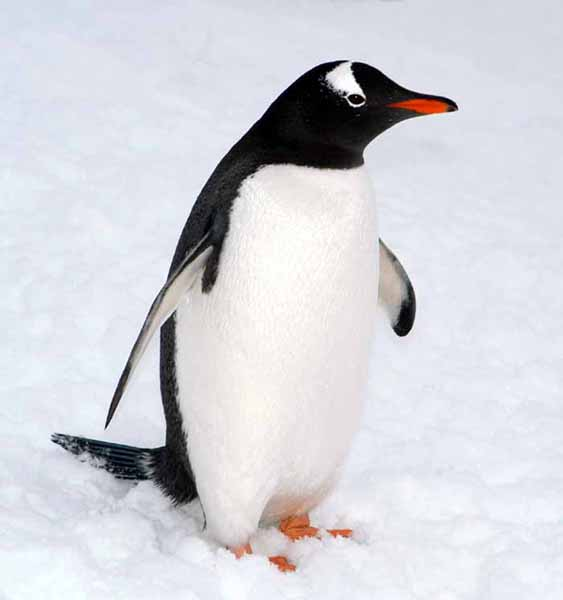
\includegraphics[width=0.7\linewidth]{./gentoo1}
\end{figure}
\end{frame}


\begin{frame}{Gentoo Linux}
\begin{itemize}
\item Sistema operacional livre baseado em Linux ou FreeBSD
\item Pode ser optimizado e personalizado de forma automática
\item Portage como administrador de pacotes
\item METAdistribuição - ferramentas para construção da tua distribuição própria e única, Gentoo power!!
\item Projeto 100\% comunitario, 7 lideres do projeto, 300 desenvolvedores, milhares de usuários
\end{itemize}
\begin{figure}[tbph]
\centering

\includegraphics[width=0.1\linewidth]{./glogo-small.png}
\end{figure}
\end{frame}

\begin{frame}{Compilação}
\begin{itemize}
\item Ebuils = Scripts com instruções para baixar, parchar, compilar e instalar pacotes com o codigo fonte
\item So baixar e instalar com pacotes muito grandes (libreoffice) ou propietarios (skype)
\item Portage como administrador da construção
\item emerge foo
\end{itemize}
\end{frame}

\begin{frame}{Compilação}
\begin{center}
¿Para que compilar se ja existem distros com pacotes prontos?
¿Vale a pena?
\end{center}
\end{frame}

\begin{frame}{Compilação}
\begin{center}
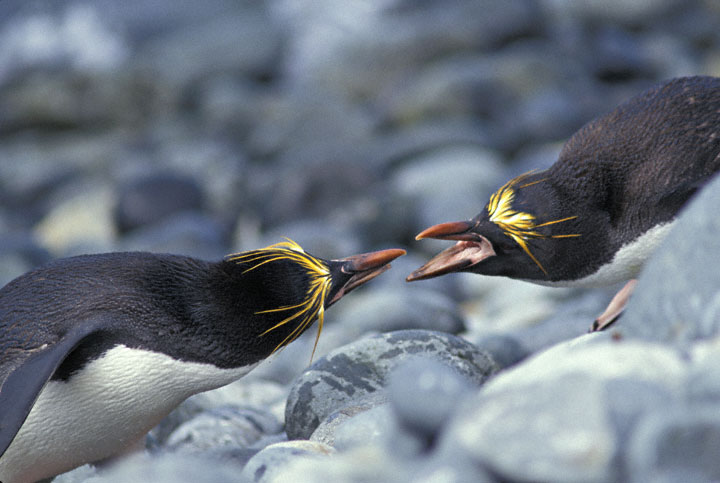
\includegraphics[width=0.7\linewidth]{./fightpen}
\end{center}
\end{frame}

\section{Mitos e realidades}
\begin{frame}{Perspectiva}
\begin{itemize}
\item 2004 - Mandrake Linux
\item 2006 - OpenSuse, Mandriva, Ubuntu, Fedora (Distro hoping)
\item 2006 - Gentoo (Usuário tempo completo)
\item 2011 - Gentoo 10 meses/Debian 2 meses
\item 2008 - Funtoo
\end{itemize}
\end{frame}

\begin{frame}{Compilação}
\begin{itemize}
\item A instalação e uma das coisas mais complicadas é mais demoradas neste mundo
\item A optimização vai fazer seu computador voar
\item Ninhem pode manter um computador com Gentoo instalado
\item Gentoo é uma distribuição muito flexível
\item Eu conheci um cara que diz que instalou Gentoo na sua cafeteira
\end{itemize}
\end{frame}


\begin{frame}{Instalação dificil}
Parcialmente certo
\begin{itemize}
\item Duas semanas :D (Celeron 1.5 Ghz, 256kbps)
\item 12 horas (Pentium 4, 512kbps)
\item 4 horas (Core i7 860, 512kbps)
\item 3 horas (Core i7 2670, 2mbps)
\end{itemize}
O aprendizagem com certeza vale a pena
\end{frame}

\begin{frame}{Optimização por compilação}
Com a configuração certa é verdade (mas nem sempre é perceptível)
\begin{figure}[tbph]
\centering
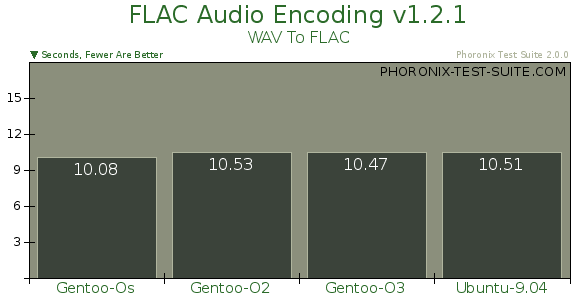
\includegraphics[width=0.7\linewidth]{./flacgentoo}
\label{fig:flacgentoo}
\end{figure}
\end{frame}


\begin{frame}{Optimização por compilação}
\begin{figure}[tbph]
\centering
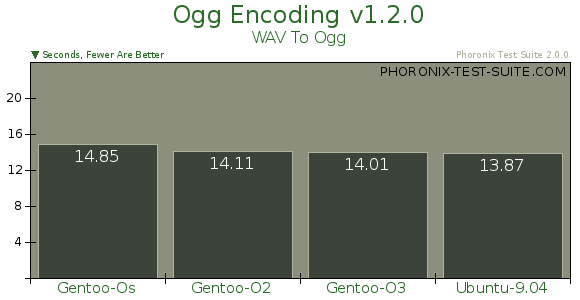
\includegraphics[width=0.7\linewidth]{./ogggentoo}
\label{fig:ogggentoo}
\end{figure}
\end{frame}

\begin{frame}{Mantenimento do sistema imposivel}
Mentira
\begin{itemize}
\item emerge -uavDN world
\item Rolling release - actualização constante
\item Nunca tive a necessidade de fazer uma nova instalação nos meus computadores 
\item Não posso celebrar versões novas porque sempre tenho a versão nova :(
\end{itemize}
\end{frame}

\begin{frame}{Gentoo Flexivel}
Verdade (namoramento)
\begin{itemize}
\item Administração atómica de dependências
\item USE flags (características selectivas)
\item Se você gosta de Gnome, quer pacotes com suporte para KDE?
\item Se você so fala português, quer instalar suporte para mandarin?
\item Precisa da documentação dos pacotes?
\item Duas maquinas virtuales de Java, três versões de python e dois compiladores C++, porque não?
\item Precisa de um kernel com todos os drivers do planeta ou so os drivers do seu computador?
\item A escolha e sua, Gentoo foi feito para ajudar!
\end{itemize}
\end{frame}


\begin{frame}{Gentoo roda em . . .}
Raspberry pi \cite{RPi2012}
\begin{figure}[tbph]
\centering
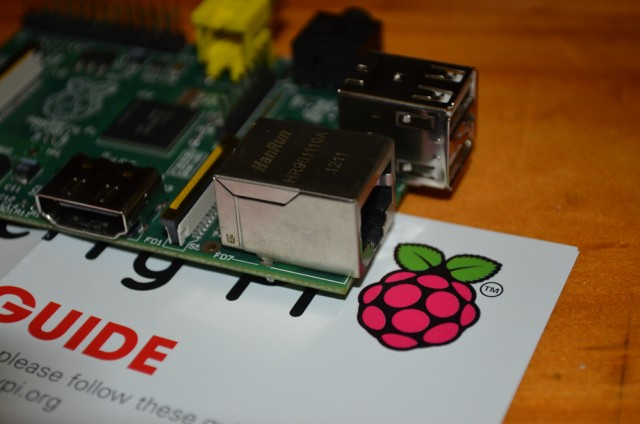
\includegraphics[width=0.4\linewidth]{./rasp}
\label{fig:rasp}
\end{figure}
Misa Digital Guitar \cite{Js2012}
\begin{figure}[tbph]
\centering
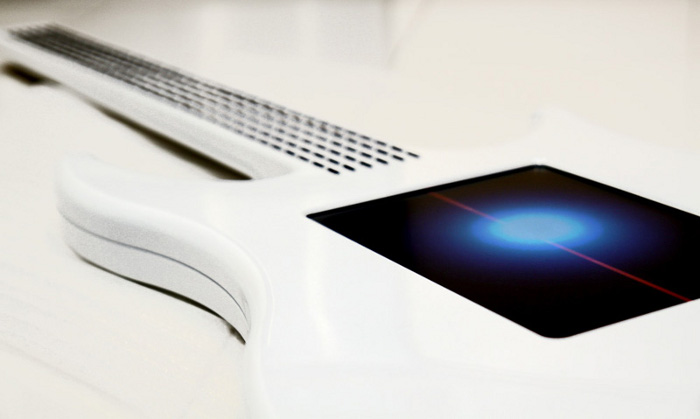
\includegraphics[width=0.4\linewidth]{./misa}
\label{fig:misa}
\end{figure}

\end{frame}

\begin{frame}{Gentoo roda em . . .}
Cluster 1200 cores e 125 nodes em Kansas State University \cite{GenClu2012}
\begin{figure}[tbph]
\centering
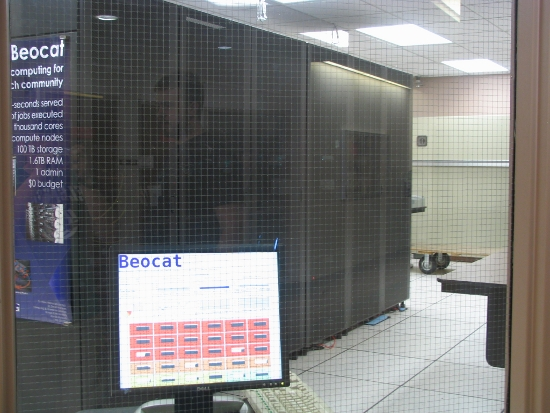
\includegraphics[width=0.4\linewidth]{./beocat}
\label{fig:beocat}
\end{figure}
Meu computador
\end{frame}

\begin{frame}{Eu quero Gentoo!}
\begin{itemize}
\item Gentoo Handbook http://www.gentoo.org/doc/pt_br/handbook/
\item Funtoo http://www.funtoo.org/wiki/Welcome
\item Sabayon http://www.sabayon.org/
\end{itemize}
\end{frame}


\begin{frame}{Obrigado!}
\begin{itemize}
\item tuxtor@shekalug.org
\item http://tuxtor.shekalug.org
\item http://github.com/tuxtor/slides
\end{itemize}
\begin{center}

\includegraphics[width=0.1\linewidth]{./cclogo}
\\
This work is licensed under a Creative Commons Attribution-ShareAlike 3.0 Brazil License.
\end{center}
\end{frame}

\section{Referencias}
\begin{frame}[allowframebreaks]{Referencias}
    \bibliographystyle{sbc}
    \bibliography{small}
\end{frame}



\end{document}